\subsubsection{Regressione}
\label{reg_1}

Procediamo ora con l'analisi del grafico del dislivello $d$ in funzione della temperatura $\theta$.
In base ai dati da noi raccolti abbiamo ottenuto il seguente risultato, illustrato in Figura \ref{fig:dislivello_temperatura}.

\begin{SCfigure}[][p]
    \centering
    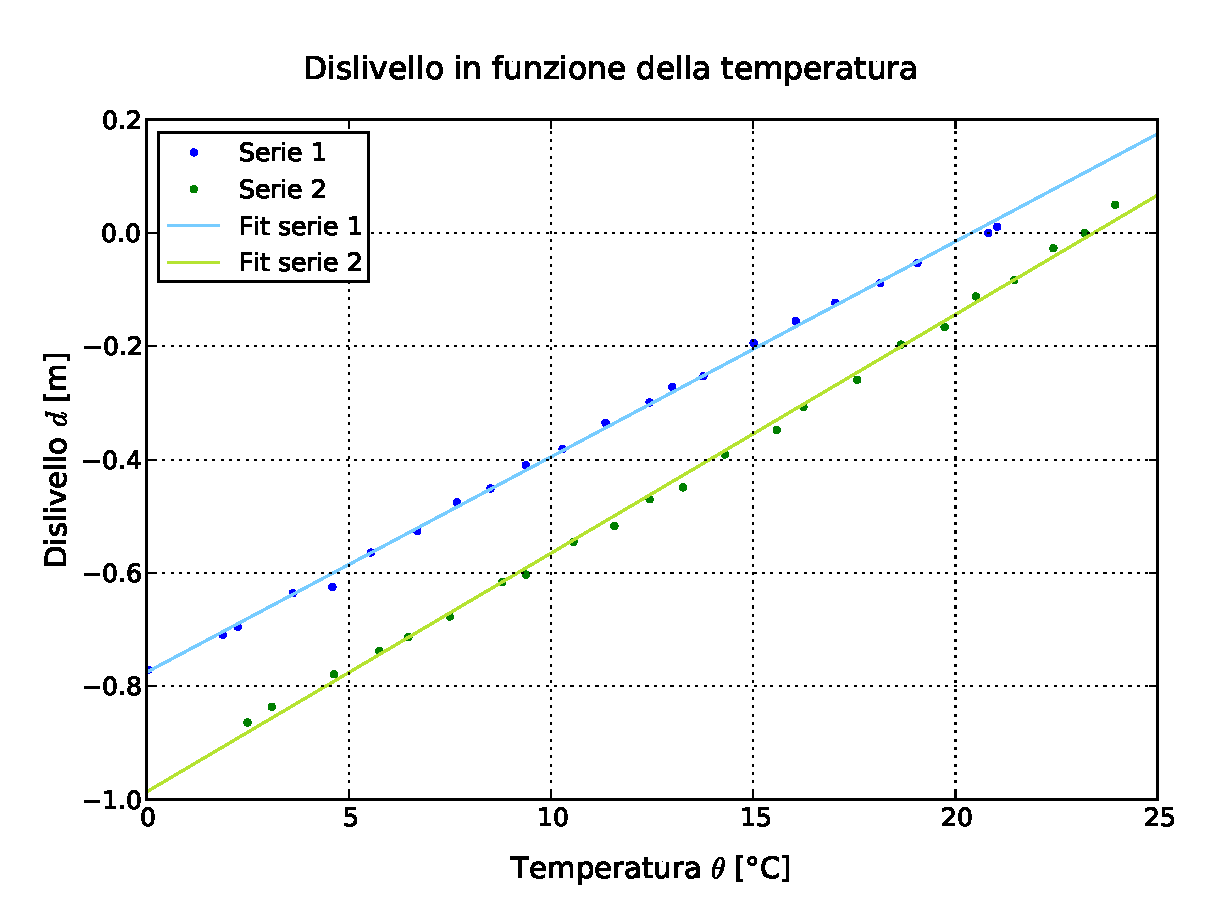
\includegraphics[width=120mm]{immagini/dislivello_temperatura.pdf}
    \caption{Grafico del dislivello in funzione della temperatura. Sono riportati i dati delle due serie con le relative
    rette ricavate dalla regressione. Non ci sono le barre d'errore in quanto sono dell'ordine di grandezza dei punti
    sperimentali, e quindi confondono solo la lettura del grafico. Si possono notare alcuni punti che deviano di parecchi
    sigma dalle rette.}
    \label{fig:dislivello_temperatura}
\end{SCfigure}
%
Si vede che esiste una correlazione tra la temperatura $\theta$ e dislivello $d$ ed è anche approssimativamente lineare.
Con il metodo dei minimi quadrati, abbiamo quindi trovato la funzione lineare

\begin{equation}
d \,=\, A + B\,\theta
\label{h_theta}
\end{equation}
%
che meglio si adatta ai dati da noi raccolti. L'intera procedura qui descritta è stata
applicata ad entrambe le serie di dati separatamente.

Come primo passo abbiamo eseguito dei fit preliminari sulle due serie di dati,
al fine di trasferire l'incertezza dalla temperatura al dislivello.
Per fare ciò occorre minimizzare la funzione

\begin{equation}
    \sum_{i=1}^{N} \frac{(d_i - A' - B'\theta_i)^2}{(\delta d)^2}
    \label{eq:min_quad}
\end{equation}
%
dove $N$ indica il numero di dati della serie, che sono $N_1 = 22$ nella prima serie e $N_2 = 23$ nella seconda.
I pedici $i$ stanno ad indicare il dato $i$-esimo della serie presa in esame. Le incertezze sul dislivello sono tutte uguali e
quindi prive di pedice.

Durante questa fase si è tenuto conto solamente dell'incertezza $\delta d$ sul dislivello. Per calcolare i minimi
di (\ref{eq:min_quad}) si sono usate le formule:

\begin{equation}
    \left(
    \begin{array}{c}
        A' \\
        B'
    \end{array}
    \right)
    =
    M^{-1}
    \left(
    \begin{array}{c}
        \sum_i d_i/(\delta d)^2 \\[2mm]
        \sum_i (\theta_i d_i)/(\delta d)^2
    \end{array}
    \right)
    \qquad
    \text{dove}
    \quad
    M =
    \left(
    \begin{array}{c c}
        \sum_i 1/(\delta d)^2 & \sum_i \theta_i/(\delta d)^2 \\[2mm]
        \sum_i \theta_i/(\delta d)^2 & \sum_i \theta_i^2/(\delta d)^2
    \end{array}
    \right)
    \label{eq:A_e_B}
\end{equation}
%
dove tutte le sommatorie vanno da 1 a $N$ e non sono stati specificati gli estremi per motivi di spazio e chiarezza. Mediante le regole
di propagazione degli errori si può calcolare che le incertezze su $A'$ e $B'$ valgono

\begin{equation}
    \delta A' \,=\, \sqrt{\frac{\sum_i \theta_i^2/(\delta d)^2}{\det(M)}}
    \qquad
    \delta B' \,=\, \sqrt{\frac{\sum_i 1/(\delta d)^2}{\det(M)}}
    \label{eq:dA_e_dB}
\end{equation}

Una volta calcolato $B'$, si è trasferito l'errore dalla temperatura al dislivello nel seguente modo

\begin{equation}
    \delta d\ped{tot} = \sqrt{\delta d^2 + (B'\delta \theta)^2}
    \label{eq:err_tras_1}
\end{equation}
%
Notare che, poiché $\delta d$ e $\delta \theta$ sono uguali per tutti i dati della serie,
anche l'errore $\delta d\ped{tot}$ è in comune a tutti i dati.

Infine si è minimizzata nuovamente la (\ref{eq:min_quad}), sempre tramite le formule (\ref{eq:A_e_B}) e (\ref{eq:dA_e_dB})
dovutamente modificate, utilizzando però $\delta d\ped{tot}$ invece che $\delta d$.
%
Si sono così ricavati i valori definitivi $A$ e $B$. La procedura è stata applica ad entrambe le serie di dati.
Le rette ottenute sono riportate nel grafico in Figura \ref{fig:dislivello_temperatura}, assieme ai dati delle due serie.
Nella seguente tabella sono riportati i risulatati dei fit preliminari e finali per le due serie.

\begin{center}
    \small
    \begin{tabular}{l c c c c c | c c c c}
        \multicolumn{10}{c}{\textbf{Parametri calcolati con la regressione}} \\
        \toprule
        & $A'$ & $B'$ & $\delta A'$ & $\delta B'$ &
        $\delta d\ped{tot}$ & $A$ & $B$ & $\delta A$ & $\delta B$ \\
        & [cm] & [\si{\centi\meter\per\celsius}] & [cm] & [\si{\centi\meter\per\celsius}] &
        [cm] & [cm] & [\si{\centi\meter\per\celsius}] & [cm] & [\si{\centi\meter\per\celsius}] \\
        \midrule
        Serie 1 & -77.57 & 3.804 & 0.02 & 0.001 & 0.04 & -77.57 & 3.804 & 0.02 & 0.001 \\
        Serie 2 & -98.68 & 4.215 & 0.02 & 0.001 & 0.04 & -98.68 & 4.215 & 0.02 & 0.001 \\
        \bottomrule
    \end{tabular}
\end{center}

Nella tabella è riportato anche il $\delta d\ped{tot}$ con l'aggiunta dell'incertezza trasferita. Risulta chiaro che l'incertezza trasferita è
trascurabile poiché il valore $\delta d\ped{tot}$ è identico a $\delta d$. Anche le incertezze sui parametri $A'$, $B'$, $A$ e $B$
non hanno subito variazioni tra i fit preliminari e le regressioni definitive.

I valori ottenuti fit finali sono compatibili con quelli ricavati dalle regressioni preliminari; infatti tutti i parametri
sono uguali entro l'incertezza per entrambe le serie di dati.
